\documentclass{article}
\usepackage{amsmath}
\usepackage{amssymb}
\usepackage[a4paper, total={7in, 9.8in}]{geometry}
\usepackage{xcolor}
\usepackage{framed}
\usepackage{enumitem}
\usepackage{graphicx}
\usepackage{tikz}
\usetikzlibrary{arrows.meta}
\usetikzlibrary{decorations.markings}
\usepackage{physics}

\usepackage{polyglossia}

\setmainlanguage{hebrew}
\setotherlanguage{english}
\newfontfamily{\englishfont}{Latin Modern Roman}
\newfontfamily{\hebrewfont}[Script=Hebrew]{Arial}
\newfontfamily{\hebrewfontsf}[Script=Hebrew]{Arial}
\newfontfamily{\hebrewfonttt}[Script=Hebrew]{Miriam Mono CLM Bold}

\setlength{\parindent}{0pt}

\title{קוונטים 2\ \textendash\ תרגיל נומרי}
\author{\begin{hebrew}דוד שם־טוב\end{hebrew}}
\date{}

\begin{document}
\maketitle

\section{מתנד הרמוני}
\begin{tabular}{|c|c|c|}
\hline
K & הפרשים סופיים & שיטת נומרוב \\
\hline
40 & 1.490164 & 1.499892 \\
\hline
80 & 1.497554 & 1.499993 \\
\hline
120 & 1.498914 & 1.499999 \\
\hline
240 & 1.499729 & 1.500000 \\
\hline
360 & 1.499879 & 1.500000 \\
\hline
480 & 1.499932 & 1.500000 \\
\hline
600 & 1.499957 & 1.500000 \\
\hline
\end{tabular}

\begin{figure}
    \centering
    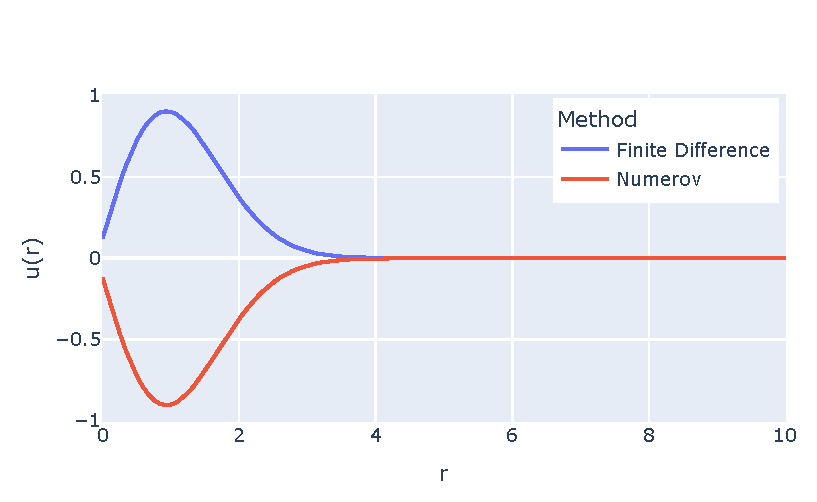
\includegraphics[width=0.5\linewidth]{plots/harmonic_oscillator/wavefunction/N120.eps}
    \caption{פונקציית הגל עבור $K=120$}
    \label{fig:wave240}
\end{figure}

\end{document}